\documentclass[preprint,10pt]{elsarticle}
\usepackage{etoolbox}
\makeatletter
\patchcmd{\ps@pprintTitle}{\footnotesize\itshape
       Preprint submitted to \ifx\@journal\@empty Elsevier
       \else\@journal\fi\hfill\today}{06.2018}{}{}
\makeatother

\usepackage[margin=2.5cm]{geometry}

\newcommand{\fscale}[1]{#1\linewidth}
\newcommand{\figref}[1]{Fig.~\ref{#1}}

%-----------------------------------------------------------------------------
%  Colors
%-----------------------------------------------------------------------------
\usepackage{pagecolor}
\definecolor{linen}{RGB}{240,240,230}
\definecolor{fwhite}{RGB}{255,250,240}
\definecolor{oldlace}{RGB}{253,245,230}
\definecolor{awhite}{RGB}{250,235,215}
\definecolor{pwhip}{RGB}{255,239,213}
\definecolor{peach}{RGB}{255,218,185}
\definecolor{ivory}{RGB}{255,255,240}
\definecolor{seashell}{RGB}{	255,245,238}

\usepackage{sectsty}
\sectionfont{\Large}
\subsectionfont{\large}

\usepackage{amsmath}
\newcommand{\mr}[1]{\mathrm{#1}}  % Roman font for the math mode
\newcommand{\mi}[1]{\mathit{#1}}  % Italic font for the math mode
\newcommand{\mc}[1]{\mathcal{#1}} % Caligrafic (script) font for the math mode
\newcommand{\ms}[1]{\mathsf{#1}}  % Sans font for the math mode (vectors and matrices)
\newcommand{\mb}[1]{\mathbf{#1}}  % Bold font for the math mode (vectors and matrices)

\usepackage{mathtools}
\DeclarePairedDelimiter\ceil{\lceil}{\rceil}
\DeclarePairedDelimiter\floor{\lfloor}{\rfloor}

\usepackage{amsthm}
\theoremstyle{definition}
\newtheorem{definition}{Definition}[section]
\newtheorem{remark}{Rule}[section]

\newtheorem{property}{Property}

\newtheorem{theorem}{Theorem}

\usepackage{cleveref}
\crefformat{section}{\textbf{\S#2#1#3}} % see manual of cleveref, section 8.2.1
\crefformat{subsection}{\textbf{\S#2#1#3}}
\crefformat{subsubsection}{\textbf{\S#2#1#3}}

\renewcommand{\cref}[1]{\textbf{\S\ref{#1}}}

\usepackage{graphicx}
\usepackage{subfigure}
\graphicspath{{./fig/}}
%% The amssymb package provides various useful mathematical symbols
\usepackage{amssymb}

\usepackage[titletoc]{appendix}
\usepackage[T1]{fontenc}

\usepackage{xcolor, soul}
\sethlcolor{oldlace}

\usepackage{lineno}
\usepackage{url}
\bibliographystyle{unsrt}

\patchcmd{\abstract}{Abstract}{Summary}{}{}

\begin{document}

\begin{frontmatter}

%% Title, authors and addresses

\title{Picolo: Fast p2p open database network\tnoteref{title1}}
\tnotetext[title1]{Version 1.2}

\author{Picolo Labs\corref{auth1}}
\cortext[auth1]{https://picolo.network}
\address{San Francisco, California}

\begin{abstract}
%% Text of abstract
Picolo is a fast, scalable, fully decentralized, globally distributed transactional database network for blockchain based applications. It is a p2p network with an open participation model where any node can freely join and leave at will. Nodes discover each other in a decentralized manner via DHTs where each node maintains just enough routing information that will enable it to discover the topology of the whole network. It uses a probabilistic replication framework on top of DHTs to achieve an O(1) lookup latency in the average case. It also adds a layer on top of DHTs that allows locating nodes by geographic regions.
\newline
\newline
All nodes in the network are symmetric - they all run the same database software that provides a number of desirable features. Clients can interact with them via a generic SQL interface that has familiar methods such as selections, aggregations and projections. Nodes typically are part of a replica group (of a small size like 5) and the network is made up of many such groups. Nodes in a replica group are responsible for the same data where mutations to it are synchronously replicated to all replicas. Mutations are applied in the order seen by nodes where order is determined by timestamps that are a combination of physical and logical clocks. This gives Picolo the property of external consistency - the strongest consistency property a database can achieve. Distributed transactions across nodes are also made possible by using these hybrid timestamps. Automatic data sharding is supported when it grows too big or for load balancing purposes. Queries posed to the network can be run across all nodes with vastly differing schemas. Overtime, semantically similar schemas are logically grouped together for faster processing and richer results. There is a notion of \textsf{user-controlled} and \textsf{app-controlled} schemas that aids in achieving data sovereignty. Fine grained access control rules to data can be defined via a declarative language which are then enforced via encryption.
\newline
\newline
There are four types of participants in the network: \textsf{storage providers}, \textsf{storage consumers}, \textsf{data providers} and \textsf{data consumers}. Storage providers join the network to offer their spare computing resources like disk space, cpu and memory in exchange for cryptographic tokens. Consumers can pay providers with these tokens (among other ways) and use the resources provided to satisfy their needs. Since the network is open for anyone to participate, consumers need some safety guarantees before they can reliably store their data on untrusted nodes. So providers are required to put up security deposits and the network is designed to be tolerant to their byzantine behavior, to punish malicious nodes by slashing their deposits and to reward honest nodes for diagnosing and reporting byzantine behavior. A mechanism called \textsf{Proof-of-Query} is used for the diagnosis and deposit slashing is enforced by a smart contract system.
\end{abstract}

\begin{keyword}
	\textsf{decentralization \sep blockchain \sep ethereum \sep database \sep sql \sep access control \sep secret sharing \sep p2p \sep tokens \sep incentives \sep mechanism design \sep byzantine faults \sep data sharing}
\end{keyword}

\end{frontmatter}

\newpage
\tableofcontents
\newpage
%-----------------------------------------------------------------------------
%  INTRODUCTION
%-----------------------------------------------------------------------------
\section{Introduction}\label{Sect:Introduction}
We are in the midst of building a new Internet. Blockchain networks like Ethereum have popularized the idea of unstoppable, owner less applications that are run on an open network of untrusted but incentivized nodes without the oversight of a central authority. An increasing number of these decentralized applications (\DJ apps) are being created everyday with evolving data storage needs. The first generation of these dapps stored their data entirely on a blockchain itself while the current ones are storing it on decentralized file storage systems like IPFS with just hashes of the data stored on the blockchain. Although this method works for dapps with simple storage needs like the need for storing data as a blob, it is very limiting for dapps with more complex requirements such as the need to store data at a more fine grained level and efficiently querying it. A popular option is then to use a cloud hosted database (ex: Google’s Cloud SQL) but that turns a dapp into a non-dapp by introducing centrality into the system. \newline\newline
In this paper we introduce \textsf{Picolo}, an open database network that combines the benefits of a traditional database and p2p software. It is the world's first NewSQL $decentralized$ database system that offers features such as a SQL interface, distributed transactions, external consistency \cite{External_Consistency}, lock-free reads and snapshot reads. It is an open network that allows anyone with spare computing power and disk space to join the network and get rewarded for hosting and serving structured data.
\newline\newline
Features that set \textsf{Picolo} apart from other decentralized databases:
\begin{itemize}
	\item Transactions can be applied across rows, columns and tables across nodes
	\item Client controlled replication and data placement
	\item Support for storage of typed data
	\item Support for semi-relational structure for tables
	\item Configurable backups and restore mechanisms
	\item Allows for verifiable transaction logs
	\item Data poisoning detection
	\item Distributed query processing
	\item Fine grained access control to data
	\newline
\end{itemize}
Rest of the paper is structured as follows: in section 2, we discuss some related work. Section 3 presents the overall design of the system, section 4 presents the network subsystem, section 5 presents the database subsystem and section 6 presents our approach to dealing with problems that arise in a network made up of untrusted nodes and discusses an incentive mechanism to make them behave as per system's needs. In section 7, we propose a message exchange protocol in the same vein as http but for relational data sharing. Section 8 concludes the paper.

%-----------------------------------------------------------------------------
%  BACKGROUND SECTION
%-----------------------------------------------------------------------------
%-----------------------------------------------------------------------------
%  BACKGROUND SECTION
%-----------------------------------------------------------------------------
\section{Related Work}
There have been attempts in the academia at building peer-to-peer data management systems (PDMS). PeerDB \cite{PeerDB} pioneered a full-fledged data management system that supports fine-grain content-based searching on a distributed network of nodes with heterogeneous schemas. It proposed a "code goes to data" paradigm where mobile agents are employed to perform query processing at a peer node in order to reduce network bandwidth. PIER \cite{PIER} provides a relational data model and query operators on top of any distributed storage system. It embraces the notion of \textit{data independence} and only concerns itself with query processing. It does not provide any sort of replication or ACID guarantees of a database and does not maintain any indexes of its own. Piazza \cite{Piazza} describes a system where peers have pairwise schema mappings between heterogeneous schemas and how these can be transitively extended to answer queries from peers separated by more than one edge. Queries are reformulated at each peer to match the local schema before execution. While this approach works well for a few reformulations, a large number of them may result in information loss or returning of irrelevant results.
\newline\newline


In the blockchain space, there are a few projects tackling the decentralized storage problem. Filecoin \cite{Filecoin}
adds an incentive layer on top of widely used IPFS \cite{ipfs} - a p2p file sharing system. It pays miners for
contributing disk space and network bandwidth to the filecoin system. Storj \cite{Storj} and Sia \cite{Sia} are two
similar projects that offer decentralized file storage systems for end users wanting to store files on more resilient,
secure and censorship resistant networks. While these networks are great for storing large unstructured files like
images, videos, documents etc they are not suitable for storing structured data and do not support complex queries
beyond simple keyword search.

    \begin{itemize}
        \item Bluezelle, fluence, pepperdb
    \end{itemize}




%-----------------------------------------------------------------------------
%  OVERALL DESIGN SECTION
%-----------------------------------------------------------------------------
\section{Overall Design}

    \begin{itemize}
        \item Overall Picolo architecture.
        \item Token economics.
    \end{itemize}




%-----------------------------------------------------------------------------
%  NETWORK SUB-SYSTEM SECTION
%-----------------------------------------------------------------------------
\section{Network Subsystem} 

The network layer is a fully decentralized, peer-peer overlay routing layer among the nodes participating in the Picolo
database network. The most important goal of the network layer is to help locate content as efficiently and quickly as
possible while surviving certain kinds of failure or malicious intent. Peer-peer networking literature refers to this
functionality as Decentralized Object Location and Routing (DOLR) \cite{dolr2003}. The network layer focuses on routing
messages, such as database queries, read/write requests or other management functions to the respective nodes which can
satisfy them. 

The overlay layer can be implemented on top of any datagram network protocol such as UDP or IP. Specifically on the
Internet, we realize its implemented on IP or IPv6 protocols.  The peer-to-peer overlay routing infrastructure offers
efficient, scalable, location-independent routing of messages directly to nearby copies of an object or service using
only localized resources \cite{tapestry2004}. We use the word object to loosely refer to content such as Tables, Shards,
Metadatd and such, that is, any content that is content-addressable and needs to be part of the lookup layer.  Location
independent routing refers to a class of techniques for locating objects based on content rather than their location,
while attempting to find the shortest path possible to reach such objects. Picolo's design offers the following
properties which are required of any high performance p2p overlay-based lookup layer:

\begin{itemize}
    \item {\em Determinstic Node Mapping}: Picolo is able to locate objects anywhere in the network. That is, there
        should be no object in the network that cannot be accessed using the lookup layer.
    \item {\em Low routing inefficiency}: Routes should have low {\em stretch}. Stretch is the ratio between (network
        level) distance traveled by a query to an object and the minimal network distance from the query to the object.
        Optimal solution would be to always send the query to the nearest copy possible.
    \item {\em Balanced load}: The load should be evenly distributed across the nodes in the network, thus, reducing
        hotspots.
    \item {\em Dynamic membership}: THe system allows arrival and departure of nodes while maintaining functionality.
\end{itemize}

-- Self-repairing.
-- Soft-state based routing.

\subsection{Background}

In this Section, we provide a brief overview of peer-peer systems both in the research and product community that have
influenced the literature over the last 20 years.

Napster \cite{Napster} was one of the first popular service that provided much of the original inspiration for peer-peer
systems although its database was centralized.  DNS is an example of a widely deployed distributed and largely
decentralized key-value database that powers every lookup and interaction on the Internet \cite{Mockapetris_1988}. DNS
relies on special root servers to bootstrap the lookup protocol. The Freenet \cite{freenet_thesis, Clarke_2001} and the
Gnutella \cite{Gnutella} p2p systems were popular in the previous decade for file sharing. Both systems were designed
for sharing of large files over a longer duration of time. Content reliabilty including lookup reliability and network
latency goals were necessary in this enviroment. 

The second generation of peer-peer systems include research driven projects such as Chord \cite{Stoica_2001}, Content
Addressable Network (CAN)
\cite{Ratnasamy_2001}, Pastry \cite{Rowstron_2001}, Tapestry \cite{tapestry2004} and
Kademlia. Chord along with CAN, Tapestry and Pastry developed the concept of distributed hash tables (DHTs) as a
fundamental mechanism for content-based addressing. They built over the scalability and self-organizing properties of
both FreeNet and Gnutella by providing a definite answer to a lookup query in a bounded number of network hops. In fact,
these protocols are able to locate content within \( O(log N) \) where \(N\) is the number of nodes in the system. From
an 
API perspective, these overlays provide a key-based routing (KBR) interface that supports deterministic routing of
messages to a live node that has the responsiblity for the "value" corresponding to the given key. These systems also
support high level APIs such as Dynamic Object Location and Routing (DOLR) \cite{dolr2003}. Most DHT's use the concept
of consistent hashing to distribute the load evenly among the nodes.

{\em Consistent hashing:}
Typical hashing based schemes do a good job of spreading load through a known, fixed collection of servers. Since the
Blockchain consists of nodes on the Internet which can appear and disappear based on incentives and other criteria, our
assumption is that machines come and go as they crash or are brought into the network. Also,
the information about what nodes are functional propagates slowly through the
network, so that clients may have incompatible “views” of which nodes are available to replicate data. (Note that a
node can also be a client). This makes standard hashing useless since it relies on clients agreeing on which nodes are responsible for serving a particular
page.

Like most hashing schemes, consistent hashing assigns a set of items to buckets so that
each bin receives roughly the same number of items.  Unlike standard hashing schemes, a small change in the bucket set
does not induce a total remapping of items to buckets. In addition, hashing items into slightly different sets of
buckets gives only slightly different assignments of items to buckets. 

Chord uses such hash functions to map nodes and content uniformly to a circular 160-bit
namespace. Chord improves the scalability of consistent hashing by removing the requirement that every node knows about
every other node. Each node only maintains about \(O (log N) \) state information about other nodes in an \( N \) node
network. When nodes join or leave, they require \( O(log^2 N) \) messages to keep the network updated.

CAN routes messages in a {\em d}-dimensional space where each node maintains a routing table with \(O(d)\) entries and
any node can be reached in \(O(dN^{1/d})\) routing hops. CAN's routing table does not grow with network size, but the
number of routing hops grows faster than \(log N\).

When compared to Chord and CAN, Pastry and Tapestry take network distances into account when constructing overlay
topologies. While Chord and CAN use shortest overlay hops and other runtime heuristics, both Tapestry and Pastry
construct locally optimal routing tables to reduce any routing inefficiencies. 

Pastry and Tapestry share some similarities to the work by Plaxton et al \cite{Plaxton_1997} and to the routing layer in
the Landmark hierarchy \cite{Tsuchiya_1988}. The approach consists of routing based on address prefixes or otherwise
called prefix-based routing. However, both Pastry and Tapestry include an ability to self-organize the network structure
and achieve network locality in content mapping which also lends support for replication.
In addition, Tapestry also allows some application-based locality management by "publishing" location pointers
throughout the network for efficiently locating content and services.

Kademlia \cite{kademlia} is another p2p DHT-based routing system that uses prefix-based routing by arranging 160-bit IDs
(node IDs and content IDs) in a binary tree style data-structure for efficient routing. It uses an XOR-based distance
metric for building the routing table and for the routing algorithm itself. In terms of its performance and other
features, it is very similar to the above systems such as Chord, CAN, Pastry and Tapestry, but it offers simplicity in
its routing and lookup algorithms which make it attrative for implementation. IPFS \cite{ipfs} uses a version of
Kademlia for locating files for decentralized applications.

Other notable systems include Viceroy \cite{viceroy} which provides logarithmic hops through nodes with constant degree
routing tables. SkipNet \cite{skipnet} uses a multidimensional skip-list data structure to support overlay routing,
maintaining both a DNS-based namesapce for operational locality and a randomized namespace for network locality. Other
overlay proposals such as Koorde \cite{koorde} and Naor et al \cite{simple_hash} attain lower bounds on local routing
state but oversimplify some of the other features. 

The third generation of P2P research includes building applications on top of these DHT systems, validating them as
novel infrastructures or tuning them for specific use cases. For example, applications such as PAST \cite{past} and
SCRIBE \cite{scribe} are built on top of Pastry. Decentralized file storage application project OceanStore \cite{oceanstore} was built
on top of Tapestry, while CFS \cite{cfs} was build on top of Chord. FarSite \cite{farsite} uses a conventional
distributed directory service and could be built on top of Pastry. Another example of an overlay network is the Overcast
System \cite{overcast}, which provides reliable single-source multicast streams.

\subsection{Design of the Picolo overlay network}

The Picolo overlay network consists of a p2p DHT based lookup for mapping key to objects, content or services. There is a caching layer that allows for frequenly used items to be propagated closer to the demand endpoints in the network including ability to replicate as needed.

\subsubsection{Picolo namespace} 
1. Nodes and content map to a single 256-bit space. We can use existing hash functions such as SHA-256 for this purpose.

This space can be segregaged using a namespace identifier, which allows multiple such "naming layers" to co-exist. For example, one way to assign naming layers could be based on a per-application type.

For the rest of this section, the discussion gets isolated to within a single naming layer.

\subsubsection{Core API}
Picolo's network layer supports an API similar to a standard p2p overlay network, for a detailed discussion refer
\cite{dolr2003}. The primary goal of the API is to publish and locate objects or service identifiers within a given
namespace. All operations that occur in a namespace can be replicated across namespaces as needed.

Currenlty, we support the following API methods in a decentralized manner:
\begin{itemize}
    \item Publish()
    \item Unpublish()
    \item Lookup()
    \item RemoteCall()
\end{itemize}

\subsubsection{Routing and Lookup}

\begin{itemize}
    \item Lookup using a prefix-based DHT. 
    \item Routing table description.
    \item Lookup algorithm.
    \item Caching links for faster lookup. 
\end{itemize}

\subsection{Node Dynamics}

Failures, node departures, node additions.

\subsection{Replication and caching}
Beehive stuff for O(1) lookups for power law queries

Structured peer-peer distributed hash tables can implement lookups in \( O(log N)\) hops. Since each hop could add between 100-500
ms of latency, for a network of 10K to 100K nodes this computes to about 4-5 seconds for a lookup (or more). Thus, we
require a caching and replication strategy to reduce this cost especially for popular items. The discussion in this
Section applies to any content or service thats is made available through the p2p system and thus extends beyond the
Database as a blockchain service provided by Picolo.

There has been significant prior work on caching and replicating strategies for peer-peer overlay networks. Methods such
as Beehive \cite{beehive} provide a closed-form replication algorithm based on a derived equation that guarantees
\(O(1)\) lookup but require full knowledge of the network, such as number of nodes and popularity values for each data
item. While this system might be good for analysis and benchmark purposes, its implementation is not pratical for
Picolo. Kelips \cite{kelips} is a probabilistic algorithm that also provides \(O(1)\) lookup performance (in the
expected case) by dividing the network into \(O(\sqrt(N))\) affinity groups each of \(\sqrt(N)\) size. They use the
gossip protocol to replicate content to all nodes within an affinity group. Work by Gupta et al \cite{one_hop_lookup}
explore the tradeoff between routing table size and lookup latency. They offer a guaranteed \(O(1)\) lookup by
maintaining routes to each and every node in the network. Farsite \cite{farsite} provides a better ttradeoff by using
routing tables of \(O(dn^{1/3})\) size to route within \(O(d)\) hops.

Other peer-peer applications such as PAST \cite{past} and CFS \cite{cfs} use fixed size caches on intermediate nodes to
cache the objects being queried. While they are unable to provide closed-form analytic bounds on query time, their
average case performance is reasonably good.

We draw on the above literature to find the right balance between routing table size, cache and replication storage at
nodes versus lookup latency. The strategy presented in this Section achieves \(O(1)\) lookup on average for networks with standard node
and popularity dynamics. In other words, we allow for node joins, failures, unexpected departures (including malicious
intent) along with changes in service or object popularity. We also allow for "flash crowds", that is, an item, object
or service (such as a table-shard, or certain rows in a table) can quickly gain popularity (as given by standard
Internet virality models \cite{virality_model}).

\begin{itemize}
    \item A node caches or replicates an item with a probability that is proportional to the number of queries it is
        expected to get for that item in the upcoming time interval T.
    \item The difference between a cache and a replica is application specific. For the Database application that the
        network layer hosts, it depends on whether a particular table or a shard is allowed to have write permissions on
        the replica.
    \item When a node caches or replicates an item, it affects the probabilitic demand distribution for the item at
        nodes that are on the routing path which would have gotten the request has this item not been cached.
    \item Thus, by repeating this algorith iteratively, it would converge to the best caching pattern which would reduce
        lookup times with high probability for all items on the network.
\end{itemize}

\subsection{P2P Connectivity protocol}

When a Picolo node starts for the first time (fresh install), it will query a set of "root" servers, similar to the DNS
architecture of the Internet which is one of the largest decentralized lookup databases in the world \cite{icann_root}. 
These root servers populate the nodes with a list of neighboring nodes and content to bootstrap with.

The nodes use QUIC for server-server connections. QUIC primer. Why QUIC ?

Certain network configuations might not allow for QUIC, such as due to firewalls. In such cases, we will use the SPDY
protocol which offers multi-session transport over the HTTPS ports which every firewall should support.

STUN/NAT traversals and proxies.

\subsection{Cryptoeconomics and Byzantine behavior}
How will malicious nodes affect the system and how to mitigate/prevent/recover. Do nodes have incentive to participate in network discovery

\subsection{Analytics and Debug/Fault diagnosis}



%-----------------------------------------------------------------------------
%  DATABASE SUB-SYSTEM SECTION
%-----------------------------------------------------------------------------
\section{Database Subsystem}
In this section, we discuss core database concepts like byzantine paxos, role of timestamps in achieving external consistency, distributed transactions and sharding. Concepts that are most new to a database network built for the  decentralized world like distributed query processing, dynamic clustering, data sovereignty and decentralized fine-grained access control are presented.

\subsection{Consensus, replication \& sharding} \label{sec:paxos}
All data on \textsf{Picolo} is replicated for durability and high availability. Storage consumers have the option of choosing a replication factor that suits their needs. They can also choose where to locate their data based on where their users are located to achieve better latency or to comply with regulations like GDPR. This data locality can easily be achieved by instructing the network layer to only allow replicas that belong to a geographic region to join the replica group. Consensus is achieved amongst replicas by a running a variant of paxos that is tolerant to byzantine faults.
 \subsubsection{Paxos based replication}
 We modify the algorithms in \cite{byzantine_paxos} to make the leader election more frequent and add a slashing condition that punishes byzantine behavior. There are two roles that each replica can take: \textsf{proposer} and \textsf{acceptor}. Proposers initiate changes to the state by proposing new commands to be appended to a \textsf{sequence} from which the replica state is generated and acceptors vote on which sequence to accept. The system moves through different \textsf{views}. A view can be thought of as a discrete time period (in the order of minutes) with a monotonically increasing view number $\textsf{view}_\textsf{num}$ and has a distinguished proposer called \textsf{leader}. If one imagines that each replica has a number from the set ${1..\mathcal{N}}$ where $\mathcal{N}$ is the number of replicas, then the leader for a view can simply be chosen as $\textsf{leader}_\textsf{view} = \textsf{view}_\textsf{num} \enspace \% \enspace \mathcal{N}$. There are two modes in which the consensus process happens: \textsf{fast} and \textsf{classic}.
\newline\newline
\textbf{Fast mode}: In fast mode (equivalently, \textsf{leaderless mode}), proposers can directly send commands to acceptors bypassing the leader. This obviates the need for \textsf{phase 1b} messages of classic paxos. In a network where replicas are present in distant geographic locations, the savings could be significant. Note that all messages are digitally signed, so the senders can be uniquely identified. A message is a tuple ($\textsf{view}_\textsf{num}$, \textsf{seq}) where \textsf{seq} consists of a prefix - the last accepted command sequence, suffixed with new commands. This differs from the classic paxos algorithm where only scalar values are passed around and offers two major advantages:
\begin{itemize}
	\item Commands need not be exactly similar - commands can appear in differing orders in different replicas as long as they are commutative.
	\item Proposers don't need a promise from acceptors that they will not accept values with a lower \textsf{ballot number} 
\end{itemize}
In the context of a database, two commands are commutative if they are mutating independent records that don't depend on each other for state calculation. For example, reading a row and writing to another row in a table are commutative operations where as reading and writing to the same row may not be. Even writing to different rows if they have different timestamps is non-commutative if \textit{external consistency} is to be maintained (\cref{sec:hybrid_time}). The relaxed definition of command similarity helps replicas achieve consensus quicker compared to the usual case. Since we cannot assume synchronicity of the network, messages may appear in different order at different replicas. So as long as they are commutative, we can tolerate the order difference and proceed with the consensus process. The acceptors always accept a sequence with the highest length, so they don't need to send back the ballot number promise.
\newline\newline
\textbf{Classic mode}: It is possible that the acceptors are unable to make progress in fast mode $i.e$ append new commands to their sequences when they receive concurrent proposals. Since the network is asynchronous and messages may reach out of order, if they are non-commutative and are of the same length, the acceptors cannot agree on the order by themselves. So they fallback to the leader to arbitrage an order for them. They send their sequences to the leader of the current view $\textsf{leader}_\textsf{view}$ who then executes a classic ballot to achieve consensus.
\newline\newline
\textbf{Byzantine fault detection}: Once acceptors receive new proposals, they first verify if the new sequence contains as a prefix an already accepted sequence by them in the past. If not, they simply reject it. If it does, then they sign their acceptance and multicast it to other acceptors. Other acceptors then perform the same check and if it passes, signal their acceptance by $appending$ their signature and multicast it again. This process continues until $\mathcal{N} - f$ acceptors each receive messages with $\mathcal{N} - f$ signatures at which point, the sequence is considered agreed upon and a message is sent back to the proposer indicating consensus. Here $\mathcal{N} \ge 3f+1$. During this process if an honest acceptor receives a multicast that contains signatures of an acceptor $\mathcal{M_A}$ on two non-commutative sequences (see \figref{fig:byz_faults}), then it will trigger a slashing condition (\cref{sec:slashing}). Since we require at least $\mathcal{N} - f$ acceptors to agree on a proposal, at least one of them is guaranteed to be honest and it will trigger the slashing condition. 
\begin{figure}[h!] \centering
	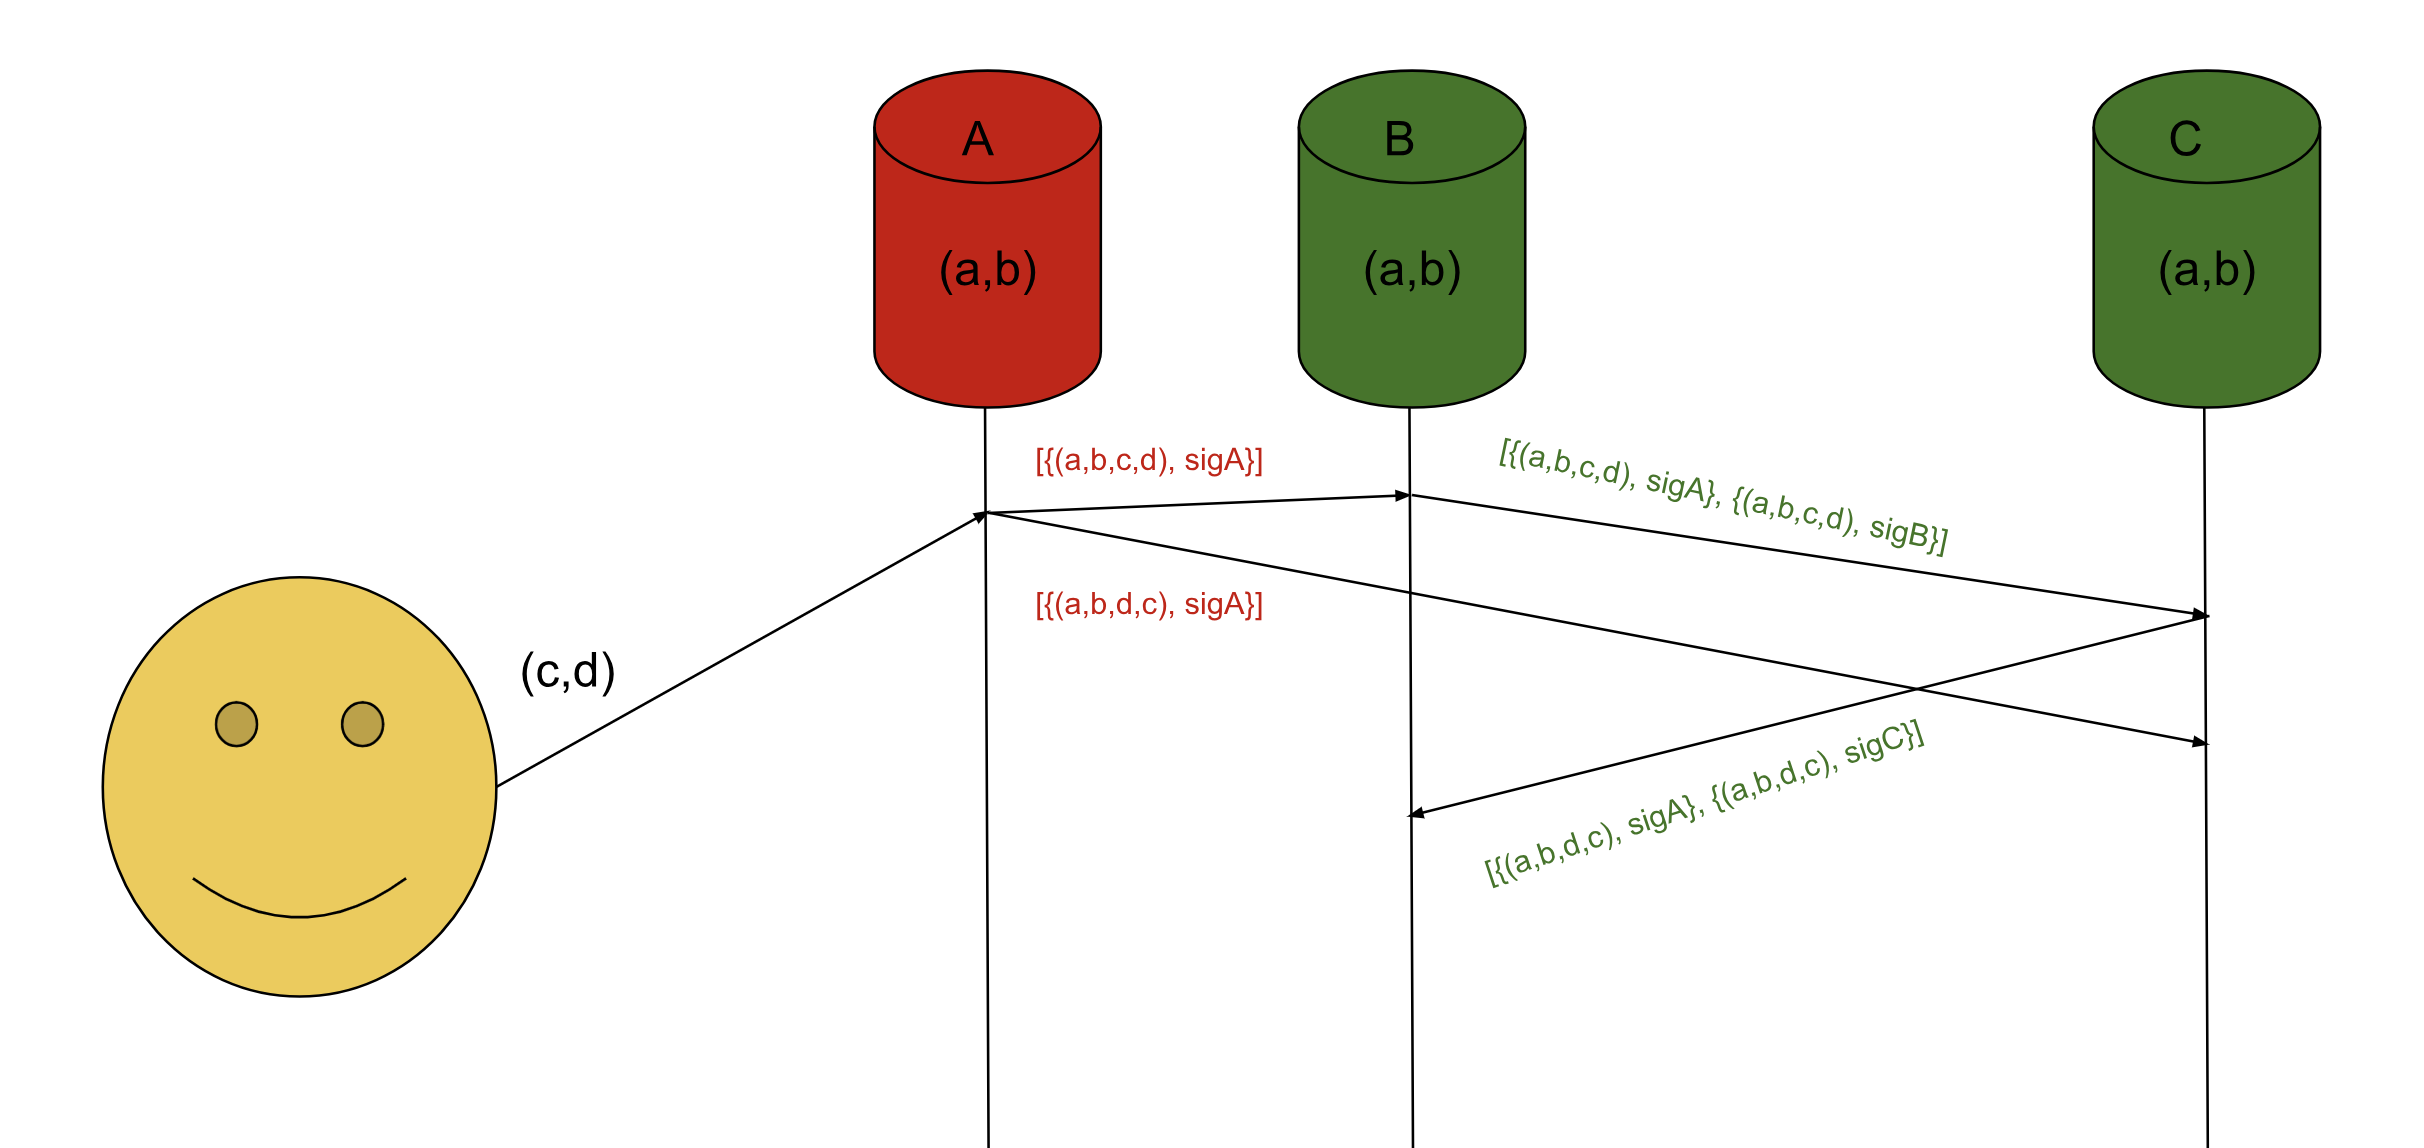
\includegraphics[width=\fscale{0.76}]{byz_faults.png}
	\caption{Byzantine fault detection during Paxos. Replica A sending conflicting messages is detected by B and C}
	\label{fig:byz_faults}
\end{figure}

\subsubsection{Sharding}
\textsf{Picolo} automatically partitions data into multiple shards when it grows too big for any one replica. Each shard consists of a set of key ranges (typically 64MB). A \textsf{key range} is the smallest atomic unit that is replicated aka governed by a paxos group. It is also the smallest unit of movement when data from one replica needs to be sharded into distinct replica sets. The process of sharding is a well studied problem in databases and implementations can be readily found, so we omit a detailed discussion here. 

\subsection{External consistency, Hybrid time \& Distributed transactions} \label{sec:hybrid_time}
Intuitively, external consistency property \cite{External_Consistency} of a distributed system guarantees that the state changes seen by it are exactly in the order applied to it by an external actor. It is the strongest form of consistency a distributed database system can offer and is notoriously hard to achieve in a system with asynchronous network links. Google's Spanner \cite{spanner} achieves this by using the TrueTime api which exposes clock uncertainty as an interval. Every transaction in Spanner has a TrueTime timestamp that indicates its time of entry into the system. Maximum clock uncertainty guaranteed by Truetime is 7ms (due to datacenter latencies); which means by making every transaction wait for 7ms before committing, Spanner can guarantee their total ordering system wide. While these low \textit{commit-wait} latencies (7ms) made possible by state of the art datacenters work fine for Spanner, a decentralized network like \textsf{Picolo} has no such luxuries and needs a new trick.
\subsubsection{Using timestamps}
\textsf{Picolo} uses hybrid time \cite{hybrid_time} - a combination of physical clocks and logical clocks for timestamping. Each node is assumed to provide an accurate enough physical timestamp by running a daemon process that syncs time with NTP stratum 1 servers like Google's external NTP service. If a node's clock is off by more than 500ms from the average of its paxos group, \textsf{Picolo} automatically kills it and finds a replacement. The logical clock is simply a monotonically increasing number appended to the physical time; so its possible to do a simple lexicographic comparison to determine relative order. For each write transaction, $\textsf{leader}_\textsf{view}$ assigns a hybrid timestamp to it before proposing it to replicas. So when two requests r1 followed by r2 hit the same paxos group and pass by $\textsf{leader}_\textsf{view}$, all the replicas are guaranteed to commit requests in the same order irrespective of the order in which they are received. For transactions that span multiple paxos groups, a coordinator (one of the $\textsf{leader}_\textsf{view}$ of individual paxos groups) is elected to perform a \textsf{2 phase commit (2PC)} with other leaders. In the \textsf{prepare} phase of 2PC, each leader acquires locks for its corresponding group and replies with its current timestamp. The coordinator then selects the highest timestamp of all the replies and uses it as the timestamp of the transaction during \textsf{apply} phase. This timestamp is also sent back to the initiator of the transaction so that it can pass it to a subsequent causally related transaction (if any). In the case where this propagation is not possible, external consistency cannot be guaranteed and application developers need to employ the commit wait strategy used by Spanner if desired, although at a performance expense.
\subsubsection{MVCC}
Multi version concurrency control (MVCC) is the practice of storing multiple versions of the same data. In \textsf{Picolo}, each record is uniquely identified by a timestamped key. So keys that differ only by their timestamps represent different versions of the same data. By keeping these different versions, \textsf{Picolo} offers such features as lock-free reads, time travel reads and snapshot isolation. Clients executing read transactions therefore need not acquire any locks since any concurrent writes on the same record have a newer timestamp and won't affect its older timestamped value. Records can also be fetched from the past by specifically executing a read transaction with an older timestamp. For writes however, a lock needs to be acquired on the key being modified. Lock status of keys is stored in a lock table and transactions that mutate data need to check whether the key/range of keys they try to operate on is already present in the lock table, in which case they need to wait. Else, they create an entry in the lock table (thereby acquiring the lock) before proceeding. Similarly, for writes spanning multiple paxos groups, one of the $\textsf{leader}_\textsf{view}$'s is chosen as the coordinator of a \textsf{2PL} (two phase locking) process that facilitates the locking of keys/key ranges of each group by its respective leader.

\subsection{Data in web 3.0}
Our long term goal for \textsf{Picolo} is to make it \textit{the} data network for web 3.0 (\cref{sect:applications}). Data in the new web will be solely controlled by data owners and resides in a single shared network. To support such a network, following capabilities must be built:
\subsubsection{Distributed query processing} \label{sec:dynamic_cluster}
A web 3.0 data network needs to have the capability to execute queries across $all$ nodes in the network in response to a client request. Since nodes will have vastly differing schemas, effective mechanisms for searching and query proessing \cite{query_reformulation, query_processing1, query_processing2} are needed. High level architecture of a \textsf{Picolo} node is depicted in \figref{fig:node_arch}.
\begin{figure}[h!] \centering
	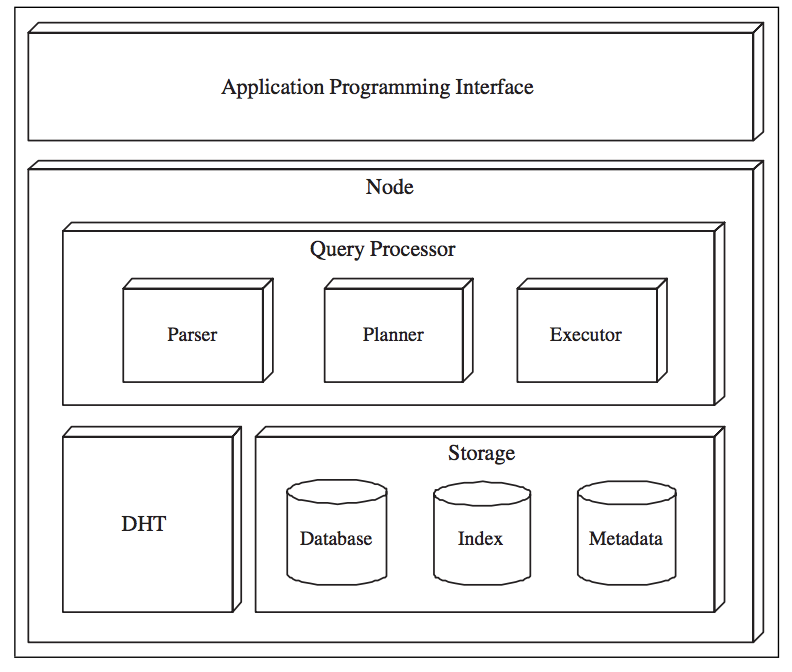
\includegraphics[width=\fscale{0.76}]{node_arch.png}
	\caption{A \textsf{Picolo} node}
	\label{fig:node_arch}
\end{figure}
The schema dictionary depicted in the figure contains metadata to be exposed to the world. Nodes that wish to keep data private should not export the data's metadata to the schema dictionary. Suppose there is a table called \textsf{users} with four columns: \textsf{username}, \textsf{firstname}, \textsf{lastname} and \textsf{email}. The exported metadata entry might look like:
\begin{center}
	\begin{tabular}{| c | c |} 
		\hline
		Entity & Keywords \\ [0.5ex] 
		\hline
		\textsf{users} & user, people, customer, profile\\ 
		\hline
		\textsf{name} & name \\
		\hline
		\textsf{firstname} & fn, {f\_name}, {first\_name} \\
		\hline
		\textsf{lastname} & ln, {l\_name}, {last\_name} \\
		\hline
		\textsf{email} & id, contact \\ [1ex] 
		\hline
	\end{tabular}
\end{center}
When a query is posed to any node in the system, the node first tries to fulfill it with a local query before passing it along to its neighbors. Remember, nodes in the system host data with heterogeneous schemas. Hence the keywords are used to find semantically similar data by assisting in query reformulations.
\newline\newline
\textbf{Dynamic clustering}:
Semantic proximity metrics \cite{PeerDB} and clustering techniques \cite{dynamic_clustering} can be used to find nodes hosting semantically similar schemas. Overtime, these nodes are discovered and are clustered together for better query performance by reducing the number of network hops required.

\subsubsection{Data sovereignty} \label{sec:access_control}
\textsf{Picolo} supports two different schema types: \textit{application controlled} and \textit{user controlled}. Applications can use user controlled schemas to put users in absolute control of data and better comply with regulations like GDPR. For example, a decentralized twitter may  want users to have control over their tweets. Users can use any third party client or \textsf{Picolo}'s official clients to interact with their tweets, effectively rendering the decentralized twitter just another client to the data albeit with better features. \newline\newline
When semantics don't allow to put user in control of data, application controlled schemas can be used. An example here would be a decentralized ticketing application where users should not be given fine grained control to selectively delete data about which tickets they bought.
\newline\newline
\textbf{Access control}:
Applications and users may want to share data with other parties but may wish to impose access controls. There are a few ways of achieving this including building an API on top of the data or using proxy re-encryption techniques. In \cite{ac_p2p_db}, a secret sharing scheme is used instead, where a party given access to encrypted data collects key shares from key holders, reconstructs the key and decrypts data for further use. Acces rules can be defined by a SQL like declarative language at any granularity desired like at the level of a single row or a cell. An example row level granularity rule looks like:\newline \newline
\texttt{SELECT  * \newline FROM users \newline WHERE email=foo@bar.com \newline NODE (SELECT nodeId FROM nodes WHERE domain=application)} \newline \newline
An example value level (only username is given access to) granularity rule looks like:\newline \newline
\texttt{ SELECT username \newline FROM users \newline WHERE email=foo@bar.com \newline NODE (SELECT nodeId FROM nodes)}\newline\newline
Here \texttt{NODE} is a new SQL clause that identifies nodes/actors in the network that have access to the data covered by the rule. Each access rule creates an ecrypted block of data. When there are overlapping rules, multiple encrypted blocks are created with associated keys. The scheme also supports updates to rules - however updates cause data re-encryption and key re-distribution. 

\subsubsection{Role of encryption}
Attribute based encryption (\textsf{ABE}) \cite{abe} was first described by Goyal et.al as a way to achieve fine grained access control on data stored with a third party. It allows attaching policies or access structures to cipher texts and allows decrypting them only if the decryption key has attributes that satisfy the access structure. As an example, in a patient-disease database, a policy could be to allow to only decrypt records where the disease is flu and only keys with the attribute \textit{flu} would be able to decrypt them. \textsf{ABE} comes in two forms: ciphertext-policy ABE (\textsf{CP-ABE}) and key-policy ABE (\textsf{KP-ABE}). In \textsf{CP-ABE}, policies are attached to ciphertexts and attributes are attached to keys whereas in \textsf{KP-ABE}, policies are attached to keys and ciphertexts are labelled with attributes. While these techniques sound promising, there don't seem to be many practical implementations of them in databases. Sieve \cite{sieve} uses \textsf{KP-ABE} to protect user data stored in files with a cloud storage provider. It uses an hybrid encryption scheme where data itself is ecnrypted using a symmetric key and metadata related to the file including its location and the symmetric key is encrypted with \textsf{KP-ABE}. A client first gets the metadata, decrypts it using a key which has a corresponding policy, downloads the file and decrypts it locally with the symmetric key. A similar technique is used in \cite{PPEHR}. The \textsf{ABE} schemes used in either of these systems seem to be secure only under a \textsf{selective-set} model which  may not be sufficient in all adversarial scenarios. Moreover, key revocation in Sieve requires re-encrypting data which may not scale well while in \cite{PPEHR}, the effectiveness of key revocation is not discussed in detail.
\newline\newline
Another body of research focuses on \textsf{ABE} schemes that are \textsf{CCA2} secure. In \cite{cca2_abe1} a \textsf{CCA2} secure \textsf{KP-ABE} scheme is proposed which is based on a \textsf{large universe} construction of another \textsf{KP-ABE} scheme. They overcome the limitations of the underlying scheme by adding a dummy on-the-fly attribute to the decryption procedure which is obtained by running a temporary message through a \textsf{chameleon hash} function. In \cite{cca2_abe2}, authors describe a scheme that is adaptively secure under the complexity assumptions of 3-prime subgroup decision problem. Their scheme allows dynamic update of policies tending itself suitable for practical use cases. But similar to Sieve, the data needs to be re-encrypted by the storage provider (albeit without sacrificing confidentiality). EASiER \cite{easier} is a system that allows for dynamic policy update without the need for data re-encryption. It uses a minimally trusted proxy that faciliates efficient access revocation and can be used in constructing practical systems that use \textsf{ABE} for access control.
\newline\newline
\textsf{Picolo} is the first system that uses \textsf{ABE} for fine-grained access control in a distributed database. It allows data owners to set access rules via the declarative language above and uses a \textsf{CCA2} secure \textsf{ABE} scheme with proxy assisted revocation. \textsf{Picolo}'s construction will be more comprehensively detailed in an upcoming paper.



\section{Mechanism design}
Since Picolo is an open network and nodes can't be trusted, a robust incentive and disincentive mechanism is required to realize its correct functioning. In this section we discuss how Picolo handles failures and malicious nodes at the database and network layers. Our mechanism design consists of these main pieces:
\begin{enumerate}
	\item Node stakes and incentives
	\item Data availability checks
	\item Paxos based byzantine consensus \cite{byzantine_paxos}
\end{enumerate}
We aim to devise Casper FFG \cite{casper_ffg} style slashing conditions based on the above.
\newline\newline
\textbf{Assumptions in the attack model}: We assume a standard Byzantine failure model, i.e., the attacker is able to make changes to the messages at the network layer on a node or alter the behavior at the database layer. The attacker is also able to coordinate the behavior of multiple nodes in real-time to achieve a desired attack scenario. We also allow for the adversary to delay communication between honest nodes so long as the adversary has the ability to do so given the topology of the overlay network (i.e. the adversary should be part of the routing path). We also assume that the attacker is computationally bound, i.e., they cannot gather enough computing resources to subvert state-of-the-art cryptographic techniques such as Elliptic curve, crypto-hash functions (such as SHA-256) or encryption schemes such as AES.
\newline\newline
\textbf{Node stake}: All nodes in the network need to have a stake in order to have any meaningful participation i.e before they can start hosting large amounts of data. They can either explicitly make a security deposit when they join thereby increasing their stake or can earn rewards overtime by serving large amounts of data (by acting as cache) and use them for making the deposit. While acting as caching nodes, they are not subject to any PoQ checks (\cref{sec:poq}). 
\newline\newline
\textbf{Byzantine behaviour at the database layer}: The central tenet of our design is to use strong cryptographic primitives to push Byzantine behavior at the database layer down to either a DoS style attack vector or to the network layer where we handle it using a combination of crypto-incentives, DHT management and detection. At the database level, each node is responsible for the standard CRUD operations for a given table (or a shard). Each such operation is protected using a cryptographic signature of the entity (dapp or user) that authorizes the request. Thus a malicious node is only able to destroy the data and not alter it. For example, every write request has a signature that certifies the request. Thus, a Merkle proof audit and signature on every table can deter any malicious manipulation of the data stored. The only attack vectors that remain are various versions of DoS style disruption, where a single node or a collection of nodes disrupt the network by delaying messages or destroying the data stored. 
\newline\newline
\textbf{Network level Byzantine behavior}: Here we discuss how to handle attack vectors where the adversary can drop network messages, delete data or both. The routing layer is based on a cryptographic DHT. Thus, it is not possible for the attacker to “choose” to store a particular shard or content. The only way an attacker can do a targeted DoS is by flooding the network with a majority of nodes such that with high probability one of the compromised nodes gets the responsibility for a targeted table or shard. This mapping includes the backup nodes, thus limiting the effectiveness of a targeted attack.
\newline\newline
\textbf{Caching and replication layer incentivizes faster network links and nodes}:
The caching and replication layer prioritizes faster network links and nodes to serve requests. Thus, nodes that are dead, unresponsive or slow will get fewer requests over time. Thus, a DoS style attack scenario will cause diminishing impact over time. While the network adapts to such a disruption, it is possible for the attacker to gain enough stake and temporarily cause a slowdown. However, their stake (or trust level) would go down and they would be responsible for fewer network functions over time essentially degrading their involvement over time.	
\newline\newline
\textbf{Detection}: It is be possible to detect such DoS style behavior quickly at the network layer since the overlay topologies tend to share many links at the layer-3 on the Internet. For example, if a node appears to delay messages at the network level while maintaining fast routes and content availability might indicate malicious intent. The detection “service” can run on the nodes with the maximum stake or trust. They can detect anomalies between different layers of a potentially malicious node and agree to reduce the trust level of that node. Such a detection service can only be thwarted if the malicious node coordinates its behavior across all observable metrics such that it appears as if it is naturally faulty. For this case, it is indistinguishable from a genuinely faulty node for all practical purposes which is handled at the DHT layer (node addition, deletion, failure modes).

\subsection{Data availability checks} \label{sec:poq}
All peers (replicas) in a database cluster constantly ping each other (once every 10 seconds) to check if they are still reachable from one another. These checks are important to ensure that the replication factor of data is always maintained and for automatic fail-over. Normally, these pings contain short meaningless data. We enhance these pings with random checks for actual data nodes are supposed to be storing. We term this \textit{Proof-of-Query (PoQ)} and nodes can prove that they are storing and serving data correctly by responding satisfactorily to PoQ pings. There are two types of PoQs: \textit{peer-PoQ or pPoQ} and \textit{client-PoQ or cPoQ} (see \figref{fig:poq})
\newline
\newline
\textbf{pPoQ}: This is the PoQ that peers (replicas) within a cluster send amongst each other. In addition to ping data, peers randomly query other peers for tiny slivers of data (typically a single column value of a row aka a single cell) and compare the results from each peer against one another and with local data. If there are disparities among the results, then the entire row is fetched along with the digital signature of the row and the public key of the signer. If the signature verification fails for the data returned by a peer, then the validating peer publishes that failure as a violation and triggers the slashing condition. Then the violating peer's deposit is slashed, with a reward going to the validating peer.
\newline
\newline
\textbf{cPoQ}: This PoQ works similar to above except that it can be triggered by any client of the network, typically the party most interested in the data hosted by the cluster (a dapp). cPoQ acts as a second level security check in case all the peers in the cluster are complicit. It is up to the clients how frequently they want to send cPoQs, the trade off being data transfer from a cluster (network egress) costs money.
\newline
\newline
\textbf{Source of randomness}: It is important to choose a good source of randomness so as to ensure queries cannot be guessed ahead in time. If one imagines the data set hosted by a cluster as a giant array and the array size is known, a simple secure random number generator that generates numbers between 0 and 1 will work. Verifiers can then simply get the record at index $ \floor{random * size} $
\newline
\newline
\textbf{Note on signatures}: In our current plan signatures are stored per row. So when a row update occurs on a specific column or group of columns, the signature needs to be recreated for the whole row. This involves fetching the whole row, applying the update, creating the signature on the new row and putting back the whole row. The data overhead with this process might prove to be too much. We are evaluating an alternate scheme where signatures are stored per cell instead using a short signature scheme like BLS \cite{bls}. Trade offs between these two schemes need to be more thoroughly evaluated.
\begin{figure}[h!] \centering
	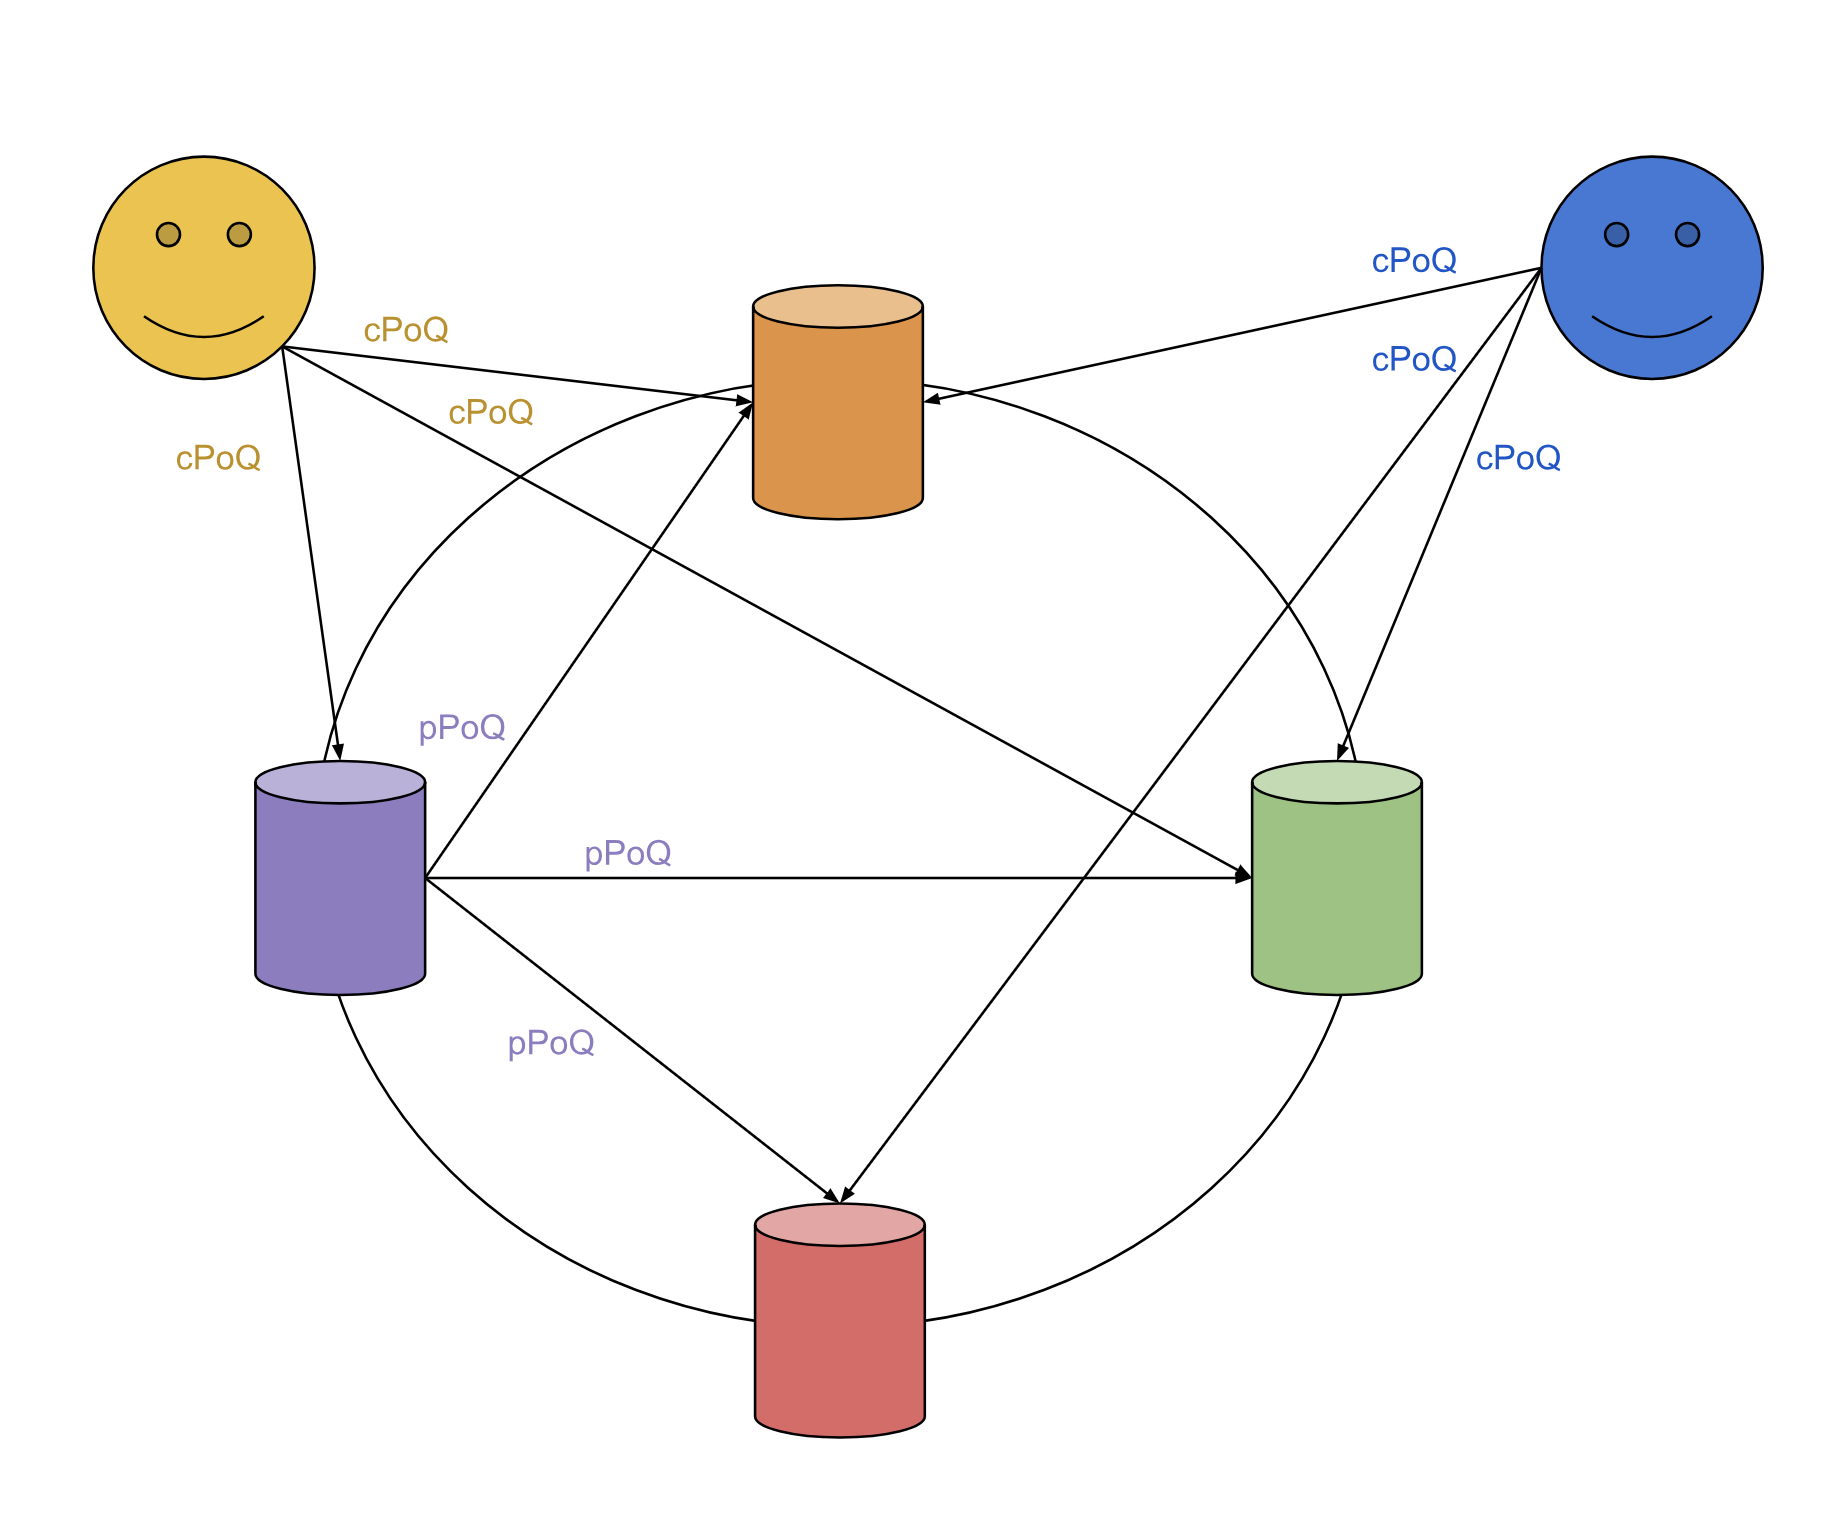
\includegraphics[width=\fscale{1}]{poq.png}
	\caption{Proof-of-Query pings}
	\label{fig:poq}
\end{figure}
 \subsection{Slashing conditions} \label{sec:slashing}
 There are three conditions, meeting any of which will result in the node losing its stake:
 \begin{enumerate}
 	\item Node found to be malicious during a paxos write
 	\item Node is continuously failing PoQ checks
 	\item Node not responding to PoQ checks
 \end{enumerate}
\textbf{Malicious behavior during paxos write}: We use a modified version of generalized byzantine paxos algorithm \cite{byzantine_paxos} for achieving replica consensus (\cref{sec:paxos}). The modified version reports back nodes in the paxos group that behaved arbitrarily during a write to the initiator of the write (client). Client can then issue cPoQs (\cref{sec:poq}) to the reported nodes and check if any data corruption occurred. It may also issue new writes and check if paxos is still reporting back arbitrary behavior of the nodes. It can then publish a proof of arbitrary behavior - simply the wrong query results (that fail signature verification) returned by the malicious nodes to a slashing smart contract that slashes deposits of malicious nodes. Malicious nodes cannot repudiate arbitrary behavior since all messages including responses to cPoQs are digitally signed.
\newline\newline
\textbf{PoQ check failure}: Similar to above, if nodes fail PoQ checks i.e return results whose signatures don't match the respective results, initiator of PoQs can publish proofs to the slashing smart contract to trigger deposit slashing. PoQs can also fail with no data returned due to a genuine hardware failure. In this case more PoQs and calls to collect file system statistics are fired to the node and if these calls indicate hardware failure, the node is simply removed from its paxos group and a replacement will be found. The node can then correct the hardware problem and join a new paxos group or simply choose to withdraw its stake and leave the network.
\newline\newline
\textbf{PoQ check unresponsiveness}: When a node has not explicitly left the network but stops responding to queries, its deposit is slowly drained. Arguably this method is more punitive than is necessary, the alternate being simply marking the node dead and finding a replacement, but stake draining acts as a deterrent to nodes going silent abruptly. It keeps the network more reliable and performant as replacing a node can be an expensive process. The function that calculates draining rate should take into account these factors:
 \begin{enumerate}
	\item Uptime of the node, $t$
	\item Amount of data on the node, $\mathcal{D}$
	\item Current load, $\ell$
	\item Rewards earned so far, $\mathcal{R}$
\end{enumerate}
The function should be inversely proportional to $t$, $\ell$ and $\mathcal{R}$ and directly proportional to $\mathcal{D}$. These relationships make sense because a node with a long uptime might need repair and is genuinely down, a node under heavy load may not be able to respond to PoQs in time as it is busy serving clients, a node that has earned a large amount of rewards so far is trustworthy as it has been serving requests correctly so far and finally since replacing a node hosting a  large amount of data is expensive, it must be penalized for going offline abruptly. Representatively,
\newline
$$ \mathcal{F}_{drain} \propto \frac{\mathcal{D}} {t * \ell * \mathcal{R}}$$
\newline
The exact function to calculate the rate of drain requires more thought and experimental evaluation with some trial \& error and hence not discussed here.

\subsection{Market design}
There are a fixed number of tokens (PINTs - PIcolo Network Tokens), all minted at genesis. They will be distributed according to a well defined plan amongst investors, developers, partners and network participants. The primary economic activity in the network is that the nodes powering the network are paid by consumers for storage, compute and network bandwidth. And the goal of our market design is to optimize towards a single goal:
\begin{center}
	\colorbox{oldlace}{\textit{\large{\textbf{Value of PINTs should increase with usage of the network}}}}
\end{center}
To that end, we propose the following mechanisms:
\subsubsection{Work token model}
In the utility token model, tokens suffer from the velocity problem. The model also requires that tokens be widely distributed aka into the hands of the consumers which could prove difficult to achieve in practice. Mandating the use of network token to pay for services also introduces friction. The user has to convert fiat to ETH/BTC first, then convert them again to the network token on a different exchange. Providers on the other hand need to again convert these tokens into more mature/liquid tokens in order to realize gains as quickly as possible as the cost of them holding on to these tokens could be higher than they like \cite{moe}. 
\newline\newline
To avoid these problems we use the work token model \cite{new_model_utility_token}: network tokens are only required for storage providers to earn the right to join the network. Anyone wishing to become a node on the network need to put up a stake in PINTs in proportion to the resources they'd be providing - more storage provided means more stake required. This stake will be slashed if they are found to be byzantine (\cref{sec:slashing}).They can then accept payment from users in any form they prefer including in PINTs. This token model also captures the value created by the network 100 \% - when the demand for the network goes up, more providers will want to join the network by purchasing PINTs to use as stake. This puts an organic upward price pressure on the token and vice-versa.
\subsubsection{Fair cooperative incentive} \label{sec:fair_incentive}
There are four types of participants in the network (\cref{sec:participants}). The inentives for storage providers and consumers are straight forward - providers get paid by consumers who are benefitting from the service. For the other two types, it is a bit more involved. While the data providers can moentize their data by imposing access controls (\cref{sec:access_control}) and charge for sharing the key information, they might not want to do that. They might be genuinely interested in sharing their data for altruistic purposes or are benefitting in a non-monetary form (e.g: by letting developers create innovative services with the data). But this leads to \textit{free riding} problem and \textit{greedy behavior} amongst nodes. Emmanuelle et. al \cite{fair_incentives} defined the \textit{fair resource sharing} problem and desgined an incentive framework that rewards nodes for acting in a way that maximizes the utility of the network. However, their design depends on a ``middleware layer" that tracks various metrics to properly incentivize and punish nodes. In addition to introducing asymmentry into the network, the tracking mechanism depends on nodes truthfully reporting metrics data. Clearly, this strong assumption will not hold well in a byzantine world as nodes can incorrectly report metrics about their peers in an attempt to damage their participation and access levels defined in \cite{fair_incentives}.
\begin{remark}{\textbf{Reply:}} \label{reply_rule}
	A node should reply to GET messages (\cref{sec:mx_protocol}) if its dataset contains records that satisfy the query in GET message.
\end{remark}
\begin{remark}{\textbf{Forward:}} \label{forward_rule}
	A node should forward GET messages with positive hop numbers to neighbors.
\end{remark}
\begin{definition}{\textbf{Semantic group:}} \label{def:sem_group}
	A semantic group is a dynamic cluster (\cref{sec:dynamic_cluster}) of peers that share semantically similar data.
\end{definition}
\begin{definition}{\textbf{Access level $\mathcal{A}\ell$:}}
	Access level of a node is the probability with which its queries will be fulfilled or other queries will be forwarded to by peers in its semantic group.
\end{definition}
\begin{definition}{\textbf{Cooperative:}}
	A node is said to be cooperative if it follows rule \ref{forward_rule}.
\end{definition}
\begin{definition}{\textbf{Fair:}}
	A node is said to be fair if it follows rules \ref{reply_rule} and \ref{forward_rule}.
\end{definition}
A rational node's objective is to keep its access level high in order to get high quality results to its queries. The access level of each node in a semantic group is tracked by all nodes in the group in a \textit{\textbf{non-interactive}} way i.e a node cannot influence what its peers think the access level of a particular node should be. There is no consensus process amongst nodes to determine a common access level value of a node. Each node determines for itself what the access levels of its peers are based on its past interactions with them. For e.g: if a node $\mathcal{A}$ has responded to a node $\mathcal{B}$'s queries satisfactorily in the past, then $\mathcal{A}$'s access level as far $\mathcal{B}$ is concerned will be high and it will respond to $\mathcal{A}$'s queries favorably in the future. Thus,
\newline
$$ \mathcal{A}_{\mathcal{A}\ell} \propto \sum_{i=0}^{n} \mathcal{N}_i[\mathcal{A}_{a\ell}] + \epsilon$$ 
where $\mathcal{N}_i$ is a node in the semantic group and $\mathcal{N}_i[\mathcal{A}_{a\ell}]$ is $\mathcal{A}$'s access level at that node and $\epsilon$ is a minimum access level all nodes have.
\newline
A new node can elect to increase its access level (the $\epsilon$) by depositing PINTs to a smart contract. Peers check the smart contract when they receive a GET message from this node for the first time and update their local information. Each node maintains three metrics that will help determine the access levels of its peers:
\begin{enumerate}
	\item The number of times a peer $\mathcal{A}$ followed \ref{reply_rule}, $num_{reply}$
	\item The number of times a peer $\mathcal{A}$ followed \ref{forward_rule}, $num_{fwd}$
	\item The ``quality of results" returned by a peer $\mathcal{A}$, $qual (0 < qual < 1)$
\end{enumerate}
$qual$ is loosely defined and its upto to each node how to calculate this value as they are the ultimate consumers of results and its in their best interest to faithfully determine it. Thus, the access level of node $\mathcal{A}$ as per a peer $\mathcal{B}$ can be represented as,
\newline
$$ \mathcal{A}_{a\ell} \propto num_{reply} * num_{fwd} * qual$$
One might notice that there is no explicit definition of a malicious node in this mechanism. This is ok since there is no way in which a node can influence its peers; it may choose to not reply or forward messages from its peers and deliberately set the access levels of its peers to 0 locally but that does not affect the functioning of the semantic group it belongs to. All nodes set the access levels of their peers purely based on their own observation. So its upto each node to choose a behavior aka the manner in which it follows the rules \ref{reply_rule} and \ref{forward_rule} that is best for its purposes.

\subsubsection{Burning games \& applications}
Games that will encourage the burning of PINTs. Since there are a fixed number of them, burning will put an upward pressure on the price. <Todo: Atleast one idea needs to be mentioned here>
Offchain storage network to store contract state. Analytics of on chain data etc.

\subsection{Attacks}
There are four types of participants in the network (\cref{sec:participants}) and a few attacks on/from each of these are discussed below. Storj \cite{Storj} also describes a few attacks that are relevant to a storage network which we touch upon. Below list is by no means exhaustive and we foresee the emergence of a living document in the future dedicated to describing attacks and their mitigations.
\newline\newline
\textbf{Cheating provider}: A storage provider who tries to pretend that they are hosting data without actually doing so. This kind of ``passive" attack is mitigated by cPOQ (\cref{sec:poq}).
\newline\newline
\textbf{Lying consumer}: A storage consumer may report that a provider is failing cPoQs when it actually isn't. To resolve this, consumers are required to report details of the supposedly failed cPoQ, provider information and give read access to the record that cPoQ is supposed to have returned. Then anyone can check whether the cPoQs are actually failing and determine whether to slash the provider's deposit or not. Practically speaking, a committe consisting of other providers is chosen at random to verify this claim and arrives at a consensus \cite{algorand}. 
\newline\newline
\textbf{DDoS on provider}: <solution>
\newline\newline
\textbf{Selective dropper}: A storage provider may selectively drop messages from consumers. If this continues for an extended period, a consumer can simply replace this provider with a new one. Since data is replicated across multiple providers, replacement of one should not create any disruption.
\newline\newline
\textbf{Egregious egress}: A storage provider may untruthfully report serving a shockingly high amount of data to consumers. Since egress earns them money, it is expected that any rational provider tries this attack. <solution>
\newline\newline
\textbf{Free rider}: A peer in a semantic group (\ref{def:sem_group}) may not reply to or forward requests. It just joined the network to gain information about the network like what queries are being sent by clients or gather data from peers while they route it to clients. This attack is mitigated by fair cooperative incentive (\cref{sec:fair_incentive})
\newline\newline
\textbf{Greedy Ganesh}: A peer in a semantic group may choose not to forward any requests to peers or forward them with client information stripped so that they can't reply to clients directly. Then once the peers return results and ask it to route them to a client, it will just combine them with results from its local database and reply to the client as if the whole result set originated from it. Clients then see this peer as a high quality peer and send future requests to it. This leads to the formation of data islands as clients will not being able to discover valuable data hosted by other peers.
\newline\newline
\textbf{Sybil, Google attack, Honest Geppetto}:
\newline\newline
\textbf{Spartacus}:
\newline\newline
\textbf{Eclipse}:
\newline\newline
\textbf{Hostage Bytes}:
\newline\newline
\textbf{Cheating owner}: Micro payments
\newline\newline
\textbf{Faithless farmer}: Non public data should be access controlled via encryption to prevent this attack. (section 5 has more details) 

\section{MX Protocol} \label{sec:mx_protocol}
Nodes in the network need to speak the same language for efficient discovery and communication of data. Hence the following message exchange scheme (see \figref{fig:mx}) is proposed similar to \cite{Protocol_Spec}. Note that the exact mapping between the following messages and underlying transport protocol is not discussed here and may change depending on the final transport protocol chosen (\textsf{QUIC} vs \textsf{TCP})
\newline
\newline
\textbf{PUT}:  A \textsf{PUT} message contains the query to be run, an optional list of nodes to run the query against and an optional max number of hops (needed in case of an empty node list). This is used for creating or updating data in the system.
\newline
\newline
\textbf{GET}: A \textsf{GET} message contains the query to be run, max number of hops, the number of results to retrieve, the mode of retrieval (pull vs push) and a transaction identifier. Client sends this to a server to retrieve results that match the query. Parameters in \textsf{GET} can be varied depending on application needs - a streaming application may choose the push mode in which server pushes data to the client as it becomes available up until the specified number is met. A latency sensitive application may choose to retrieve a small number of results in a batch in one pull.
\newline
\newline
\textbf{SEND}: Servers respond to each \textsf{GET} message with one or more \textsf{SEND} messages with results. In pull mode, there is only one \textsf{SEND} message followed by an \textsf{END} message where as in push mode there are multiple \textsf{SEND} messages followed by an \textsf{END} message.
\newline
\newline
\textbf{END}: Servers send \textsf{END} messages to clients to indicate that they have finished sending all results in response to a particular \textsf{GET} message.
\newline
\newline
\textbf{CLOSE}: A client can send a \textsf{CLOSE} message to the server to indicate that it no longer is interested in the remaining query results and close the transaction. It doesn't have to wait until all the results are retrieved.
\newline
\newline
\textbf{OK}: Server sends this message to a client as a positive acknowledgment to a client's message.
\newline
\newline
\textbf{ERROR}: Server sends this message to a client as a negative acknowledgment to a client's message.
\begin{figure}[h!] \centering
	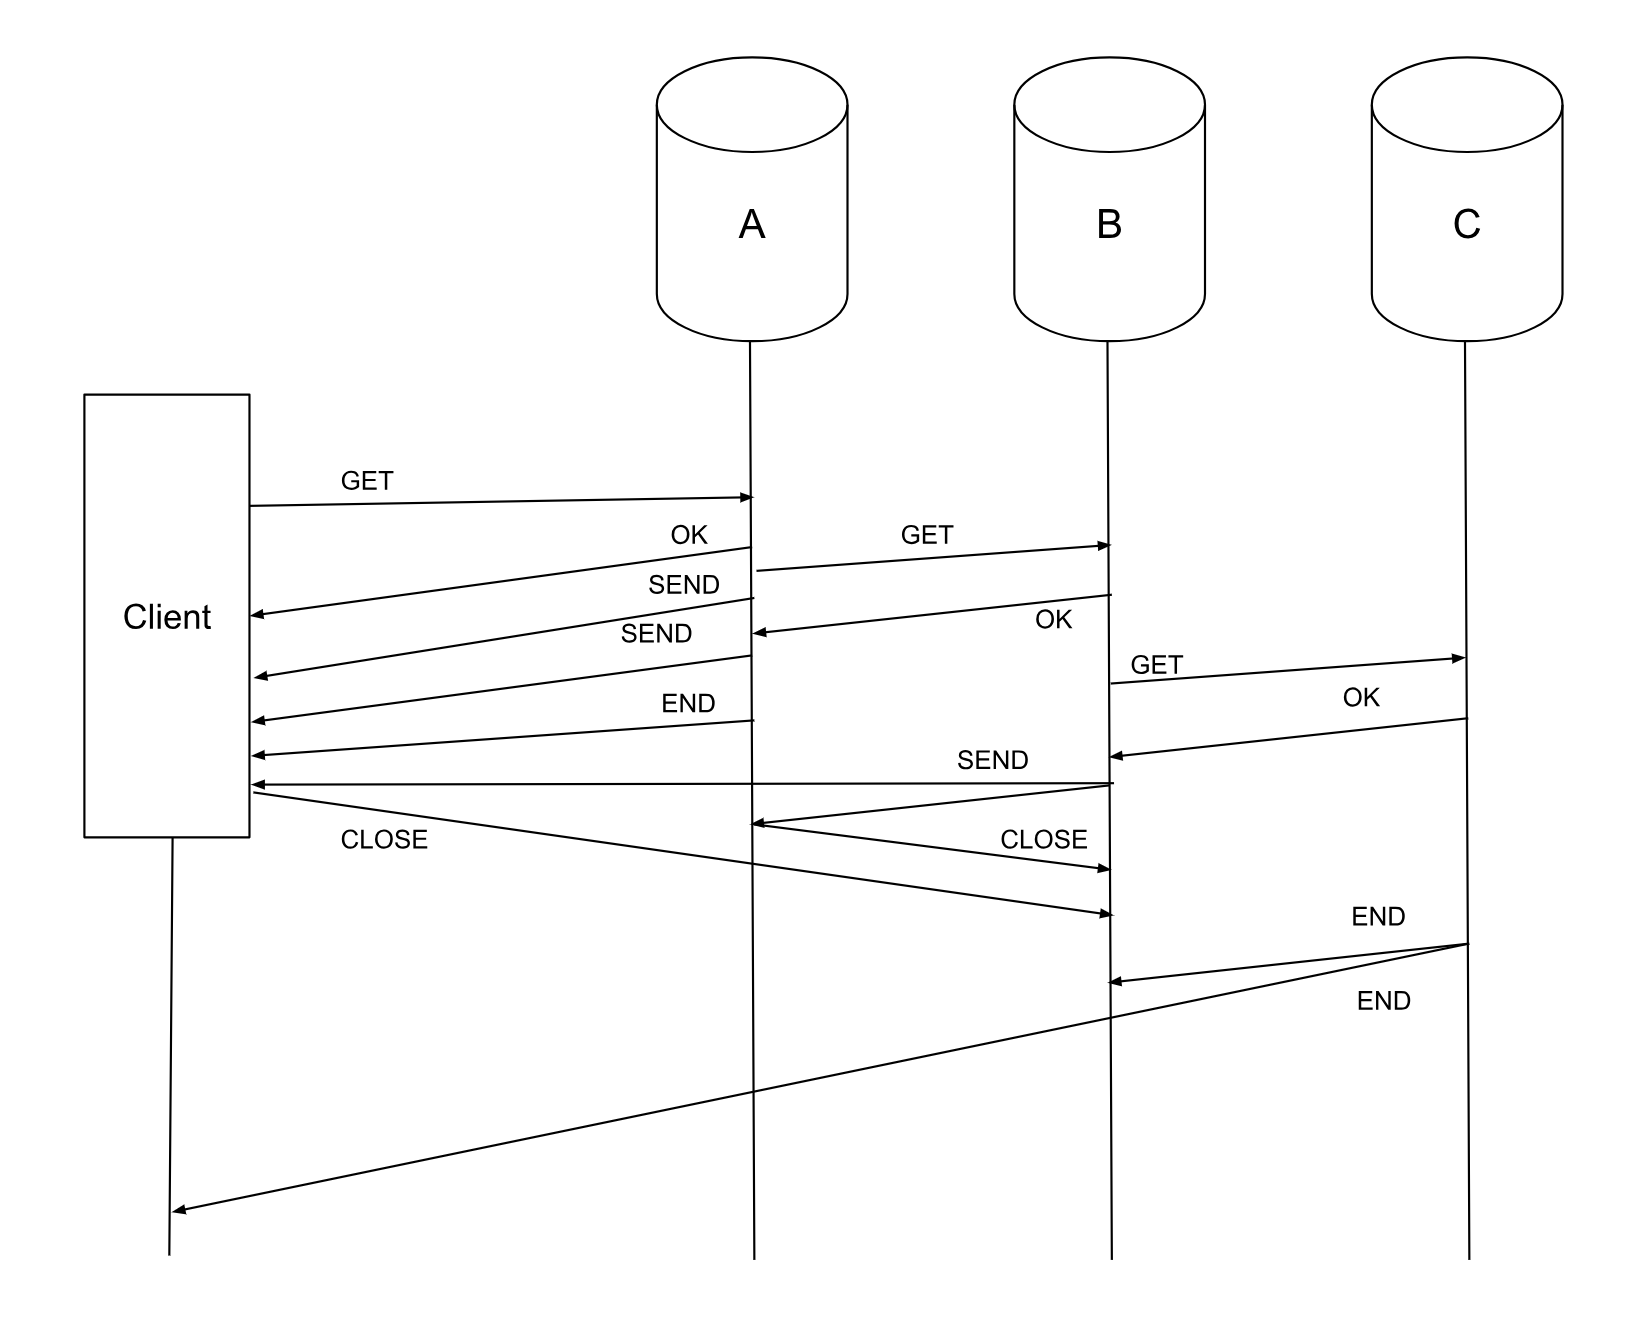
\includegraphics[width=\fscale{0.76}]{mx1.png}
	\caption{\textsf{GET} message flow, time increasing from top to bottom}
	\label{fig:mx}
\end{figure}

%-----------------------------------------------------------------------------
%  CONCLUSIONS
%-----------------------------------------------------------------------------
\section{Conclusions and Future work}
We described a database network that serves as the backbone for web 3.0 data. The network is made up of homogeneous nodes that self-organize into a p2p network based on DHTs and run a database software that provides features such as SQL interface, external consistency, auto-sharding of data and self-replication in case of failures. The network is incentive-compatible and has mechanisms in place for rewarding desirable behavior and punishing malicious intent. The network can be used by blockchain apps to store their contract state or normal apps to store generic application data and put the data owner in complete control. We discussed mechanisms to ensure data confidentiality, integrity, availability and a scheme to provide fine grained access control. We listed various attacks that are possible on the network and their respective mitigation/prevention measures.
\newline\newline
We leave the practical construction and performance analysis of attribute-based encryption scheme for a future paper. Methods to detect access control leakage, more robust defenses against DDos and Sybil attacks are left as a future exercise. A more generic access control framework based on functional encryption \cite{functional_encryption} that promises increased privacy and seems to be a step towards the holy grail of fully homomorphic encryption \cite{FHE} will also be explored in the future.
%-----------------------------------------------------------------------------
%  BIBLIOGRAPHY
%-----------------------------------------------------------------------------
\section{References}
\bibliography{./bib/picolo.bib}

\newpage

\begin{appendices}

\section{EIP-1729. Introduce SQL semantics to EVM <WIP>}
We are contemplating an EIP (Ethereum Improvement Proposal) to give Ethereum dapp developers a new choice for data storage. Not all data need to be replicated on every full node of Ethereum as the need for strongest security maybe an overkill for most smart contracts. Such data can be stored on \textsf{Picolo} network at a contract defined replication factor. Specifically, the EIP plans to introduce SQL primitives like selections, projections, aggregates etc directly into solidity (feasibility currently being evaluated).
\newline
\newline
\textsf{Picolo} may also be used by ``stateless clients'' and ``state minimized clients'' to query for data that is normally hosted by ``archival nodes'' in the current implementation or in the upcoming sharded implementation. \textsf{Picolo}'s SQL capabilities make it easy for clients to construct complex queries that are not currently possible in the simple key-value lookups provided by the EVM (Ethereum Virtual Machine).
\newline\newline
\texttt{<Mapping of SQL commands to EVM/eWASM opcodes to be defined here. Or maybe just a library contract or other ``listener'' mechanism will be easier to implement>}
\end{appendices}


\end{document}
